\documentclass{beamer}
\usepackage{graphicx} % Required for inserting images
\usepackage[colorlinks=true, allcolors=blue]{hyperref}
\usepackage{polski}
\usepackage{amsmath,amsfonts,amssymb}
\usepackage{verbatim}
\usepackage{multirow}
\usetheme{Simple}

\newcommand{\textoperatorname}[1]{%
  \operatorname{\textnormal{#1}}%
}%niby polskie znaki w trybie matematycznym

% ------------- Creating a new block template ----------
\makeatletter
\def\th@newblock{%
  \normalfont 
  \def\inserttheoremblockenv{exampleblock}}
\theoremstyle{newblock}
\newtheorem{exercise}[theorem]{Ćwiczenie}
\makeatother
%-----------------Scaling inside math mode (bigger symbols) -----------------
\usepackage{environ}

\NewEnviron{HUGE}{% 
    \scalebox{1.7}{$\BODY$} 
}

\usepackage{physics}
%---------------numbering equations in align*----------(one number to whole block)
\newcommand\numberthis{\addtocounter{equation}{1}\tag{\theequation}}

\title[short title]{Tryb matematyczny}
\subtitle{Warsztaty \LaTeX \ 2025}
\author{Dominik Piasecki}
\date{Dzisiaj}


\begin{document}

\begin{frame}
    \titlepage
\end{frame}

\begin{frame}{Github}
    \centering
    \large
    github.com/NKFSUJ/LaTeX2025
\end{frame}

\begin{frame}[fragile, c]{Po co to wszystko?}
      
    \begin{columns}
        \column{0.5\linewidth}
            \begin{figure}
                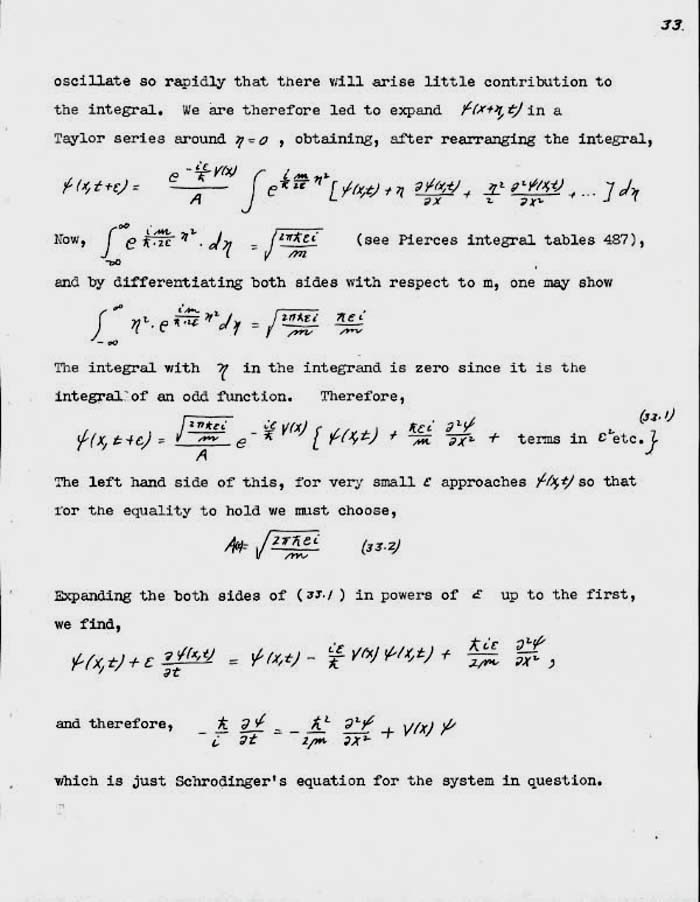
\includegraphics[width=\linewidth]{Feynmann_phd.jpg}
                \label{fig:feynman}
            \end{figure}
        \column{0.5\linewidth}
             \begin{itemize}
                \item Aby nie pisać prac, które wyglądają tak
                \item Przenoszenie wzorów z obliczeń (np. Mathematica) do dokumentów 
                \item System zapisu stosowany w notacji matematycznej na Wikipedii
            \end{itemize}
    \end{columns}

\end{frame}

\begin{frame}[fragile=singleslide]
    \frametitle{Jak zacząć używać trybu matematycznego?}
    
    \begin{itemize}
        \item \textbf{Pakiety}, które należy załączyć -  w preambule:\\
        {\centering \verb|\uspackage{amsmath, amsfonts, amssymb}|}
        \item \textbf{Tryb inline} - wstawianie równań do tekstu - równanie ograniczone znakami \verb| $...$| lub \verb| \( ... \) |
        \item \textbf{Tryb blokowy} - równania wstawiane oddzielnie, na szerokość całej linii. Automatyczna numeracja równań, możliwość odwołania do równania w teście, podpisu, wiele opcji środkowania
    \end{itemize}
        
    \begin{verbatim}
        \begin{equation*}
            [tutaj kod równania]
        \end{equation*}
    \end{verbatim}

    
    \begin{itemize}
        \item Dużą część znaków wyświetla się tak samo jak w kodzie:
    \end{itemize}
        
    \centering
    \begin{tabular}{l|l}
        \verb|$(a + b)c = ab + bc$| & $(a + b)c = ab + bc$ \\
        \verb!$|x + 3| = 7$!& $|x + 3| = 7$ 
    \end{tabular}

\end{frame}
\newcounter{cwiczenia}


\newcommand\showmycounter{\addtocounter{cwiczenia}{1}\thecwiczenia}

\begin{frame}[fragile=singleslide]
    \frametitle{Ćwiczenie \showmycounter \ - pierwsze równanie}
    Zaimportuj do dokumentu pakiety \verb|amsmath, amsfonts, amssymb|. Zapisz poniższe równania, jedno w trybie inline (\verb|$ treść równania $|) a drugie w blokowym ( \verb|\begin{equation} ... \end{equation}| )
    
    \begin{examples}
        \begin{equation}
            | x + y | < |x| + |y|
        \end{equation}

        \begin{equation}
            (a + b) c = ac + bc
        \end{equation}
    \end{examples}
\end{frame}

\begin{frame}[fragile=singleslide]{Ćwiczenie \arabic{cwiczenia} - pierwsze równanie}

    \begin{examples}
        \begin{verbatim}
$ | x + y | < |x| + |y| $
        \end{verbatim}
    \end{examples}
    \begin{examples}
\begin{verbatim}
\begin{equation}
    (a + b) c = ac + bc
\end{equation}
\end{verbatim}
    \end{examples}
\end{frame}

\begin{frame}[fragile=singleslide]

    \frametitle{Tryb inline i blokowy - różnice}

    \begin{itemize}
        \item Miejsce generowania równania - w tekście albo w osobnej linii
        \item Wygląd i skala niektórych wyrażeń:
        
        
        \begin{center}
            \begin{tabular}{c c}
                inline & blokowy \\
                
                 $\frac{1}{2}$ & $\displaystyle \frac{1}{2}$\\
            \end{tabular}
        \end{center}
        
        \item Pozycja wskaźników sumacyjnych

        \begin{center}
        
            \begin{tabular}{c c}
                inline & blokowy \\
                
                 $\sum_{n=1}^{\infty} \frac{1}{2n} = 1 $ &
                 \(\displaystyle \sum_{n=1}^\infty  \frac{1}{2n} = 1 \) \\
            \end{tabular}
            
        \end{center}
        \item W trybie blokowym możliwość tworzenia odwołań do równań, automatyczna numeracja (\verb|\begin{equation}|)
        \item Uproszony tryb blokowy - bez numeracji, brak możliwości odwołania, podpisu - \verb|\begin{equation*}|
    \end{itemize}
\end{frame}

\begin{frame}[fragile]
    \frametitle{Indeksy}
        \begin{itemize}
            \item Po każdym wyrażeniu (znaku) można wprowadzić osobno górny i dolny indeks
        \end{itemize}
        \begin{columns}[onlytextwidth, c]
            \centering
            \column{.5\linewidth}
                \centering
                \verb|[wyrażenie]^| \verb|[górny indeks]| \verb|_[dolny indeks]| 
            \column{.5\linewidth}
                \centering
                \begin{equation*}
                    [\textoperatorname{wyrażenie}]^{[\textoperatorname{górny indeks}]}_{[\textoperatorname{dolny indeks}]}
                \end{equation*}
        \end{columns}
        \vspace{0.5cm}
        \pause
        \begin{itemize}
            \item Prosty przykład
        \end{itemize}
        \begin{columns}
            \centering
            \column{.5\linewidth}
                \centering
                \verb|F_G|
            \column{.5\linewidth}
                \centering
                \pause
                $F_G$
        \end{columns}
        \begin{columns}            
            \column{.5\linewidth}
                \centering
                \pause
                \verb|F_grawitacji|
            \column{.5\linewidth}
                \pause
                \centering
                $F_grawitacji$
        \end{columns}
\end{frame}

\begin{frame}[fragile]{Grupy znaków}
    \begin{itemize}
        \item Znaki zbierane są w "grupy" używając nawiasów klamrowych
        \item Każda grupa traktowana jest jako jeden, duży znak
    \end{itemize}
    \pause
    \begin{columns}
            \centering
            \column{.5\linewidth}
                \centering
                \verb|F_|\verb|{grawitacji}|
            \column{.5\linewidth}
                \pause
                \centering
                $F_{grawitacji}$
        \end{columns}
\end{frame}
\begin{frame}[fragile]{Indeksy zagnieżdżone}
        \begin{itemize}
            \item Jedno wyrażenie nie może mieć dwóch indeksów dolnych 
        \end{itemize}

        \begin{columns}[onlytextwidth, c]
            \column{.5\linewidth}
                \centering
                    \verb| [wyr]_a_n|
            \column{.5\linewidth}
                \centering
                \alert{Błąd kompilacji}
        \end{columns}

        \begin{itemize}
            \item Aby uzyskać indeksowany indeks należy wstawić całe wyrażenie jako indeks
        \end{itemize}
        \begin{columns}[onlytextwidth, c]
            \column{.5\linewidth}
                \centering
                    \verb| [wyr]_{a_n}|
            \column{.5\linewidth}
                \begin{equation*}
                    [wyr]_{a_n}
                \end{equation*}
        \end{columns}
        
\end{frame}

\begin{frame}[fragile]{Ćwiczenie \showmycounter - indeksy}
    \centering
    \verb|[wyrażenie]^| \verb|{[górny indeks]}| \verb|_{[dolny indeks]}| 
    
    \begin{examples}
        \begin{equation}
            F_{grawitacji} = m g
        \end{equation}
    \end{examples}
    \begin{examples}
        \begin{equation}
            e^{2^{2^{2^{2}}}}_{ij}
        \end{equation}
    \end{examples}
    \begin{examples}
        \begin{equation}
            (*) \quad A_{ijk} {}^{klm} 
        \end{equation}
    \end{examples}
\end{frame}

\begin{frame}[fragile]{Ćwiczenie \arabic{cwiczenia} - indeksy - rozwiązania}
    \centering
    \verb|[wyrażenie]^| \verb|{[górny indeks]}| \verb|_{[dolny indeks]}| 
    
    \begin{examples}
        \centering
        \begin{verbatim}
            F_{grawitacji} = m g
        \end{verbatim}
    \end{examples}
    \begin{examples}
        \centering
        \begin{verbatim}
            e^{2^{2^{2^{2}}}}_{ij}
        \end{verbatim}
    \end{examples}
    \begin{examples}
        \centering
        \begin{verbatim}
             A_{ijk} {}^{klm} 
        \end{verbatim}
    \end{examples}
\end{frame}

\begin{frame}[fragile]{Ułamki}
    \begin{itemize}
        \item Składnia
    \end{itemize}
    \begin{columns}[onlytextwidth,c]
        \column{0.5\textwidth}
            \centering
            \verb|\frac{licznik}{mianownik}|
        \column{0.5\textwidth}
            \centering
            \begin{equation*}
                \frac{licznik}{mianownik}
            \end{equation*}
    \end{columns}
    \begin{itemize}
        \item Ułamki piętrowe - do licznika/mianownika należy wstawić ułamek
    \end{itemize}
    
\end{frame}

\begin{frame}[fragile]{Ćwiczenie \showmycounter - ułamki}
    \centering
    \verb|\frac{licznik}{mianownik}| 
    
    \begin{examples}
        \begin{equation}
            \frac{\frac{a}{2} + \frac{b}{2}}{2}
        \end{equation}
    \end{examples}
    \begin{examples}
        \begin{equation}
            x_1 = \frac{- b - (b^2 - 4ac)^\frac{1}{2}}{2}
        \end{equation}
    \end{examples}

\end{frame}

\begin{frame}[fragile]{Ćwiczenie \arabic{cwiczenia}  - ułamki - rozwiązania}
    
    \begin{examples}
        \begin{verbatim}
            \frac{\frac{a}{2} + \frac{b}{2}}{2}
        \end{verbatim}
    \end{examples}
    \begin{examples}
        \centering
        \begin{verbatim}
            x_1 = \frac{ - b - (b^2 - 4ac)^\frac{1}{2} }{2}
        \end{verbatim}
    \end{examples}

\end{frame}


\begin{frame}[fragile]{Znaki specjalne}
    \begin{itemize}
        \item Klawiatura ma tylko ileś (mało) symboli
        \item Chcemy pisać litery greckie  - $\varepsilon, \xi, \pi$, operatory matematyczne: $\nabla, \partial, \otimes$, inne śmieszne znaczki $  \triangleq $
        \vspace{0.25 cm}
        \pause
        \item Litery greckie i hebrajskie \verb|\litera| np:
    \end{itemize}
    
    \begin{columns}
        \column{}
        \verb|\pi|
        \verb|\aleph|
        \column{}
        $\pi$
        $\aleph$
    \end{columns}
    \pause
    \begin{itemize}
        \item Wyróżnienia za najlepszą nazwę:
    \end{itemize}

    \begin{columns}
        \column{0.5 \linewidth}
        \centering
        \verb|\wedge| \verb|\vee|

        \verb|\in | \verb|\ni|
        
        \verb|\cap| \verb|\cup|
        \column{0.5 \linewidth}
        \centering
        $\wedge$ $\vee$

        $\in$ $\ni$

        $\cap$ $\cup$
    \end{columns}
\end{frame}

\begin{frame}[fragile]{Jak znaleźć nazwę znaku?}
    \begin{columns}[onlytextwidth,c]
        \column{0.5\linewidth}
            \begin{figure}
                \centering
                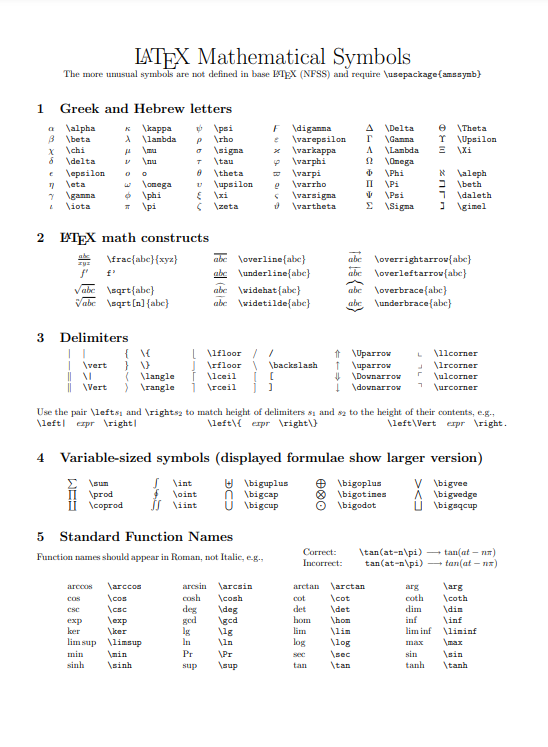
\includegraphics[width=\linewidth]{Latex_math_symbols.png}
                \label{fig:latex_math_symbols}
            \end{figure}
        \column{0.5\linewidth}
            \begin{itemize}
                \item Wyszukać \verb|LateX math symbols| i wejść w pierwsze lepsze
                \item Strony, które rozpoznają znak na podstawie rysunku - np. \textit{detexify.kirelabs.org}
            \end{itemize}
            \begin{figure}
                \centering
                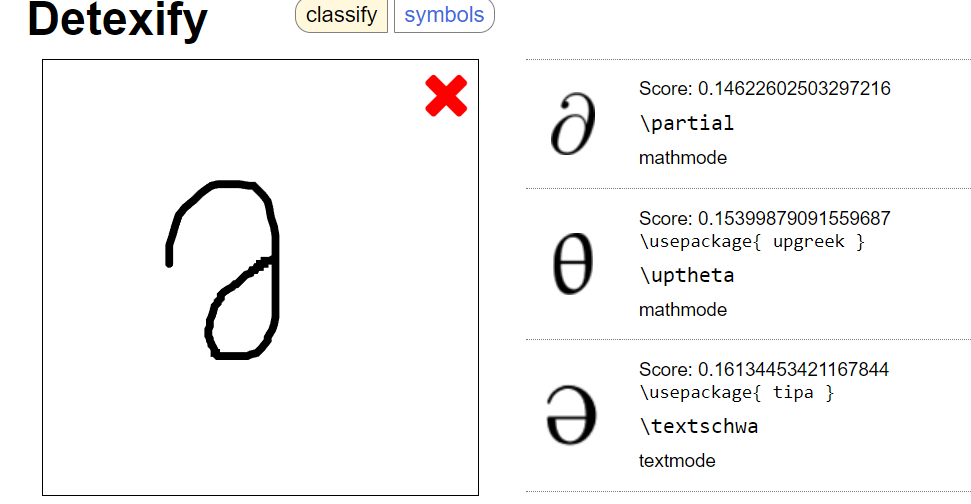
\includegraphics[width=0.9\linewidth]{Detexsify.png}
                \label{fig:detexify}
            \end{figure}
    \end{columns}
\end{frame}

% \begin{frame}[fragile]{Ćwiczenie \showmycounter \ - znaki specjalne}
%     \centering
%     LaTeX math symbols
    
%     \textit{detexify.kirelabs.org}
    
%     \begin{examples}
%         \begin{equation}
%             \varepsilon_{ijk} \varepsilon_{klm} = \delta_{jl}\delta_{km} - \delta_{kl}\delta_{jm}
%         \end{equation}
%     \end{examples}
%     \begin{examples}
%         \begin{equation}
%             x_1 = \frac{- b - (b^2 - 4ac)^\frac{1}{2}}{2}
%         \end{equation}
%     \end{examples}

% \end{frame}


\begin{frame}[fragile]{Oznaczenia funkcji}

\begin{itemize}
    \item Oznaczenia funkcji mają zdefiniowane symbole i należy je razciachować (slashować)
\end{itemize}
% \begin{columns}[onlytextwidth]
%     \column{0.5\linewidth}
%     \centering
%     \alert{Źle:} \verb|sin|

    
%     Dobrze: \verb|\sin|
%     \column{0.5\linewidth}
%     $sin$

%     $\sin$
% \end{columns}

\begin{table}[0.8\linewidth]
    \centering
    \begin{tabular}{l l l}
        \alert{Źle} & \verb|sin| &  $sin$\\
         Dobrze & \verb|\sin| & $\sin$ 
    \end{tabular}
\end{table}
\pause
\begin{itemize}
    \item Przykłady zdefiniowanych oznaczeń funkcji i innych symboli wieloznakowych:
\end{itemize}
\begin{table}[]
    \centering
    \begin{tabular}{l l l l l l}
       $\sin$ & \verb|\sin| &  $\exp$ & \verb|\exp|& $\max$ & \verb|\max|\\
       $\cos$  & \verb|\cos|&  $\log$ & \verb|\log|& $\min$ & \verb|\min|\\
       $\tan$  & \verb|\tan|&  $\lim$ & \verb|\lim|& $\limsup$ & \verb|\limsup|\\
       $\ctg$  & \verb|\ctg|&  $\arccos$ & \verb|\arccos|& $\ker$ & \verb|\ker|\\
    \end{tabular}
    \label{tab:funkcje_razciachowane}
\end{table}
\pause
\begin{itemize}
    \item Użycie funkcji razciachowanej w kodzie
\end{itemize}

\begin{columns}

    \column{0.5\linewidth}
        \centering
        \verb|\sin (x + 2k\pi)|
    \column{0.5\linewidth}
    $\sin( x + 2k \pi )$ 

\end{columns}
    
\end{frame}

\begin{frame}[fragile]{Ćwiczenie \showmycounter \ - znaki specjalne}

    \centering
    Wstawiane znaku - \verb|\nazwa|

    Nazwy znaków - \textit{detexify.kirelabs.org}

    \begin{examples}
        \begin{equation}
            \varepsilon_{ijk} \varepsilon_{klm} = \delta_{jl}\delta_{km} - \delta_{kl}\delta_{jm}
        \end{equation}
    \end{examples}

    \begin{examples}
        \begin{equation}
            \sin ^2 (\varphi) + \cos^2 (\varphi) = 1
        \end{equation}
    \end{examples}

    \begin{examples}
        \begin{equation}
            x \times y = (x \wedge y)^*
        \end{equation}
    \end{examples}

    \begin{examples}

        \begin{equation}
            \sinh(x) = \frac{e^x - e^{-x}}{2}
        \end{equation}
    \end{examples}
\end{frame}
\begin{frame}[fragile]{Ćwiczenie \arabic{cwiczenia} - znaki specjalne - rozwiązania}

    
    Wstawiane znaku - \verb|\nazwa|

    Graficzne wyszukiwanie znaków - \textit{detexify.kirelabs.org}

    \begin{examples}
        \verb|\varepsilon_{ijk} \varepsilon_{klm}| \verb| = \delta_{jl}\delta_{km}| \verb|- \delta_{kl}\delta_{jm}|
    \end{examples}

    \begin{examples}
        \begin{verbatim}
            \sin ^2 (\varphi) + \cos^2 (\varphi) = 1
        \end{verbatim}
    \end{examples}

    \begin{examples}
        \begin{verbatim}
            x \times y = (x \wedge y)^*
        \end{verbatim}
    \end{examples}

    \begin{examples}

        \begin{verbatim}
            \sinh(x) = \frac{e^x - e^{-x}}{2}
        \end{verbatim}
    \end{examples}
\end{frame}

\begin{frame}[fragile]{Znaki używające szczególnego indeksowania}
    \begin{itemize}
        \item Znak sumy, całki:
    \end{itemize}
    \begin{columns}[onlytextwidth,c]
        \column{0.5\linewidth}
            \centering
            \verb|\int_a^b| \verb|\iiint| \verb|\oint_V|

        \column{0.5\linewidth}
            \begin{equation*}
                \int_a^b \quad \iiint \quad \oint_V
            \end{equation*}

    \end{columns}
    

    \begin{columns}[c]
        \column{0.5\linewidth}
            \centering 
            \verb|\sum _ {n=1}^{\infty} n|
        \column{0.5\linewidth}
            \begin{equation*}
                \sum _ {n=1}^{\infty} n
            \end{equation*}
    \end{columns}

    \begin{columns}[c]
        \column{0.5\linewidth}
            \centering 
            \verb|\bigcup _ {n \in \mathbb{N}} K(0,n)|
        \column{0.5\linewidth}
            \begin{equation*}
                \bigcup _ {n = 1}^\infty \mathrm{K}(0,n)
            \end{equation*}
    \end{columns}

    

    \begin{itemize}
        \item Granice
    \end{itemize}

    \begin{columns}
        \column{0.5\linewidth}
            \centering
            \verb|\lim{n \rightarrow \infty}}|
        \column{0.5\linewidth}
            \centering
            \begin{equation*}
                \lim_{n \rightarrow \infty}
            \end{equation*}  
    \end{columns}

    \begin{itemize}
        \item Pierwiastek (n - tego stopnia)
    \end{itemize}
    
    \begin{columns}
        \column{0.5\linewidth}
            \centering
            \verb|\sqrt[n]{x}|
        \column{0.5\linewidth}
            \centering
            $\sqrt[n]{x}$  
    \end{columns}
\end{frame}


\begin{frame}{Ćwiczenie \showmycounter \ - wszystkie znaki specjalne}

    Graficzne wyszukiwanie znaków - \textit{detexify.kirelabs.org}
    
    % \begin{examples}
    %     \begin{equation}
    %         i \hbar \frac{\partial}{\partial t}\Psi = H \Psi
    %     \end{equation}
    % \end{examples}
    \begin{examples}
        \begin{equation}
            e^x  = \sum_{k=0}^\infty \frac{1}{k!}x^k
        \end{equation}
    \end{examples}
    
    % \begin{examples}
    %     \begin{equation}
    %         \int_{\partial M} \omega = \int_M \mathrm{d}\omega
    %     \end{equation}
    % \end{examples}

    % \begin{examples}
    %     \begin{equation}
    %         u(z) = \sqrt{(\frac{\partial f}{\partial x_1}  u(x_1))^2 + (\frac{\partial f}{\partial x_2} u(x_2))^2 }
    %     \end{equation}
    % \end{examples}

    % \begin{examples}
    %     \begin{equation}
    %         \int_{x_1}^{x_2} \sec (x) dx = \int_{x_1}^{x_2} \frac{\sec ^ 2 (x) + \tan(x)\sec(x)}{\sec(x) + \tg(x)}dx
    %     \end{equation}
    % \end{examples}

    \begin{examples}
        \begin{equation}
            \gamma = \lim_{n \rightarrow \infty} ( \sum_{k=1}^{n} \frac{1}{k} - \ln n ) = \int_0^\infty(\frac{1}{|x|} - \frac{1}{x})dx
        \end{equation}
    \end{examples}
\end{frame}

\begin{frame}[fragile]{Ćwiczenie \arabic{cwiczenia} - wszystkie znaki specjalne - rozwiązania}


    % \begin{examples}
    %     \begin{equation}
    %         i \hbar \frac{\partial}{\partial t}\Psi = H \Psi
    %     \end{equation}
    % \end{examples}
    \begin{examples}
        \begin{verbatim}
            e^x  = \sum_{k=0}^\infty \frac{1}{k!}x^k
        \end{verbatim}
    \end{examples}
    
    % \begin{examples}
    %     \begin{verbatim}
    %         \int_{\partial M} \omega = \int_M \mathrm{d}\omega
    %     \end{verbatim}
    % \end{examples}

    % \begin{examples}
    %     \begin{verbatim}
    %         u(z) = \sqrt{(\frac{\partial f}{\partial x_1}  u(x_1))^2 + (\frac{\partial f}{\partial x_2} u(x_2))^2 }
    %     \end{verbatim}
    % \end{examples}

    % \begin{examples}
    %     \begin{verbatim}
    %         \int_{x_1}^{x_2} \sec (x) dx = 
    %         \int_{x_1}^{x_2} 
    %         \frac
    %         {\sec^2(x) + \tan(x)\sec(x)}
    %         {\sec(x) + \tg(x)}dx
    %     \end{verbatim}
    % \end{examples}

    \begin{examples}
        \begin{verbatim}
            \gamma = 
            \lim_{n \rightarrow \infty} 
            ( \sum_{k=1}^{n} \frac{1}{k} - \ln n ) = 
            \int_0^\infty 
            (\frac{1}{|x|} - \frac{1}{x})dx
        \end{verbatim}
    \end{examples}
\end{frame}

\begin{frame}[fragile]{Dekoratory}

    \begin{itemize}
        \item \textbf{Akcenty} - symbole, które wywołane przed wyrażeniem będą wyświetlały się nad nim
        
    \begin{columns}
        
        \column{0.3\linewidth}
            \centering
            \verb|\vec x| $\vec x$ 
        \column{0.3\linewidth}
            \centering
            \verb|\dot \varphi | $\dot \varphi$
        \column{0.3\linewidth}
            \centering
            \verb|\tilde{xy} | $\tilde {xy}$
    \end{columns}

    \item \textbf{Strzałki}

    \begin{table}[]
        \centering
        \begin{tabular}{l l}
             \verb|\leftarrow| & $\leftarrow$ \\
             \verb|\Leftarrow| & $\Leftarrow$\\
             \verb|\leftrightarrow| & $\leftrightarrow$\\
             \verb|\Leftrightarrow| & $\Leftrightarrow$\\
             \verb|\mapsto| & $\mapsto$
        \end{tabular}
        \label{tab:strzałki}
    \end{table}

    \item{\textbf{Wielokropki}}

    \begin{table}[]
        \centering
        \begin{tabular}{l l l}
            \verb|\cdot| & $\cdot$ & np. $\vec x \ \cdot \ \vec y$ \\
            \verb|\ldots| & $\ldots$ & np. $ i_1, \ldots, i_s$
        \end{tabular}
        \label{tab:wielokropki}
    \end{table}
    
    \end{itemize}
\end{frame}


\begin{frame}[fragile]{Nawiasy}
        \begin{itemize}
        \item Nawiasy - automatyczne dostosowanie wielkości
    \end{itemize}
        \centering
        \verb|\left( ... \right)|

    \begin{itemize}
    \item Możliwość zmiany typu nawiasu przez zamianę znaku \verb|'('| 
    

    \begin{columns}
        \column{0.5\linewidth}
            \centering
            \verb|\left[ ... \right]|
        \column{0.5\linewidth}
            \begin{equation*}
                \left[ \frac{0}{\infty}\right]
            \end{equation*}
    \end{columns}
    
    \item Środowisko wymaga zawsze domknięcia nawiasów. Jeżeli nie chcemy tego robić, należy nawias sztucznie domknąć  - \verb|\right.|

    
    \begin{columns}
        \column{0.5\linewidth}
            \centering

            \verb|\left{ ... \right.|
            
        \column{0.5\linewidth}
            \begin{equation*}
                \left\{ \frac{0}{\infty}\right.
            \end{equation*}
            
    \end{columns}
    \begin{columns}
        \column{0.5\linewidth}
            \centering

            \verb|\left{ ...|
            
        \column{0.5\linewidth}
            
            \alert{unclosed begin\{equation*\} found at ...}
    \end{columns}
    \end{itemize}
\end{frame}

\begin{frame}[fragile]{Macierze}
    \begin{itemize}
        \item Czyli po prostu tabelki w trybie matematycznym
        \item Składnia
    \end{itemize}
        
    {\centering
    \verb|\beggin{array}{kolumny}| rząd 1 \verb|\\| rząd 2 \verb|\\| ... \verb|\end{array}|
    }   
    \begin{columns}
        \column{0.5\linewidth}
                \centering
                \begin{verbatim}
                \begin{array}{c c}
                    1 & 0 \\
                    0 & 1
                \end{array}
                \end{verbatim}
        \column{0.5\linewidth}
                \centering
                \begin{equation*}
                      \begin{array}{cc}1 & 0 \\ 0 & 1 \end{array} 
                \end{equation*}
    \end{columns}
    \begin{itemize}
        \item Klasyczna macierz - należy otoczyć macierz nawiasami
    \end{itemize}

    \begin{columns}
        \column{0.5\linewidth}
                \centering
                \begin{verbatim}
                \left(
                \begin{array}{c c}
                    1 & 0 \\
                    0 & 1
                \end{array}
                \right)
                \end{verbatim}
        \column{0.5\linewidth}
                \centering
                \begin{equation*}
                      \left( \begin{array}{cc}1 & 0 \\ 0 & 1 \end{array} \right) 
                \end{equation*}
    \end{columns}
\end{frame}

\begin{frame}[fragile]{Macierze - inne zastosowania}
    \begin{itemize}
        \item Macierzy można też używać w innych kontekstach, na przykład rozpisując przypadki
    \end{itemize}
    \begin{columns}
        \column{0.5\linewidth}

\begin{verbatim}
|x^2 - 1| = 
    
    \left\{
    \begin{array}{l l}
        x^2 - 1 & x \leq -1\\
        1 - x^2 & -1 < x < 1\\
        x^2 -1 & 1 \leq x
    \end{array}
    \right.
\end{verbatim}
        \column{0.5\linewidth}
            \begin{equation*}
                |x^2 - 1| = 
                \left\{
                \begin{array}{l l}
                    x^2 - 1, & x \leq -1\\
                    1 - x^2, & -1 < x < 1\\
                    x^2 - 1, & 1 \leq x
                \end{array}
                \right.
            \end{equation*}
    \end{columns}

    \begin{itemize}
        \item Klamra - użycie tylko nawiasu otwierającego (zamknięcie \verb|\right.|)
    \end{itemize}
%     \begin{itemize}
%         \item Albo podstawiając przy całkowaniu
%     \end{itemize}
%  \begin{columns}
%         \column{0.5\linewidth}

% \begin{verbatim}
% |x^2 - 1| = 
    
%     \left\{
%     \begin{array}{l l}
%         x^2 - 1 & x \leq -1\\
%         1 - x^2 & -1 < x < 1\\
%         x^2 -1 & 1 \leq x
%     \end{array}
%     \right.
% \end{verbatim}
%         \column{0.5\linewidth}
%             \begin{equation*}
%                 \int \frac{x}{x^2 + 1} dx = 
%                 \left|
%                 \begin{array}{l}
%                     u = x^2 + 1\\
%                     du = 2x dx
%                 \end{array}
%                 \right|
%                 = \frac{1}{2} \int \frac{1}{u} du = \ln |u| + C
%             \end{equation*}
%     \end{columns}

\end{frame}


\begin{frame}[fragile]{Ćwiczenie \showmycounter \ - macierze i nawiasy klamrowe}
    \begin{examples}
        \begin{equation}
            \det
            \left(
                \begin{array}{cc}
                    a & b \\
                    c & d
                \end{array}
            \right)
            = ad - bc
            \label{wyznacznik}
        \end{equation}
    \end{examples}
    
    \begin{examples}
        \begin{equation}
           f(x) = 
            \left\{
            \begin{array}{ll}
                x^2 + 3x +2  & x \leq 0 \\
                \sin(x) + 2 \ln(x) & 0 < x
            \end{array}
            \right.
            \label{funkcja_skladana}
        \end{equation}
    \end{examples}
    
\end{frame}
\begin{frame}[fragile]{Ćwiczenie \arabic{cwiczenia} - rozwiązania \eqref{wyznacznik} }
    \begin{examples}
        \begin{verbatim}
            \det
            \left(
                \begin{array}{cc}
                    a & b \\
                    c & d
                \end{array}
            \right)
            = ad - bc
        \end{verbatim}
    \end{examples}
    
\end{frame}

\begin{frame}[fragile]{Ćwiczenie \arabic{cwiczenia} - rozwiązania \eqref{funkcja_skladana} }
    
    \begin{examples}        
        \begin{verbatim}
           f(x) = 
            \left\{
            \begin{array}{ll}
                x^2 + 3x +2  & x \leq 0 \\
                \sin(x) + 2 \ln(x) & 0 < x
            \end{array}
            \right.
        \end{verbatim}
    \end{examples}
    
\end{frame}

\begin{frame}[fragile]{Co robić jak coś się nie razciachuje - fonty}

    \begin{itemize}
        \item Wybrane fonty dostępne w środowisku matematycznym:
        
        \begin{tabular}{l l}
            
        Kaligraficzne \verb|\mathcal{...}| & $\mathcal{A \ B \ C \ D \ E \ F \ G \ \ldots}$\\
    
        Mathbb \verb|\mathbb{...}| & $\mathbb{N \ Z \ Q \ R \ C \  \ldots }$\\
    
        Zmienne (domyślny tekst) \verb|\mathrm{...}| & $\mathrm{A \ B \ C \ D \ E \ F}$

        \end{tabular}

        \item Symbole, które nie są zdefiniowane

        \begin{tabular}{l l l }
             Zbiory liczbowe & \verb|\mathbb{N, \ R}| & $\mathbb{N, \ R}$\\
             Funkcje własne  &  \verb|\mathrm{err}|  & $\mathrm{err}$\\
        \end{tabular}
        
        \begin{equation*}
            \HUGE{dx \neq \mathrm{d}x}
        \end{equation*}
        
        \item Głupi sposób pisania pochodnych
        \begin{columns}
            \column{0.5\linewidth}
            \centering
            \verb|\frac{\mathrm{d}x}{\mathrm{d}t}|
            \verb|\frac{\partial x}{\partial t}|
            \column{0.5\linewidth}
                \begin{equation*}
                    \frac{\mathrm{d}x}{\mathrm{d}t}
                \end{equation*}
                \begin{equation*}
                    \frac{\partial x}{\partial t}
                \end{equation*}
        \end{columns}
    \end{itemize}
   
\end{frame}

\begin{frame}[fragile]{Wyrównywanie równań - równania równe i równiejsze}

    \begin{itemize}
        \item Środowisko \verb|\begin{align}| lub \verb|\begin{align*}|

        \item Znak \verb|'&'| symbolizuje miejsce, w którym równania mają zostać wyrównane

        \item Znak \verb|'\\'| oznacza miejsce, w którym ma nastąpić przejście do nowej linii

        \item Możliwość wstawienia wielu znaków \verb|'&'| - zachowanie analogiczne do tabeli
    \end{itemize}

    \begin{columns}
        \column{0.5\linewidth}
        \centering
\begin{verbatim}
\begin{align}
    x^2 + 10 x + 3  &= -18\\
    x^2 + 10 x + 21  &= 0\\
    (x + 3)(x + 7) &= 0
\end{align}
\end{verbatim}
        \column{0.5\linewidth}
            \begin{align*}
                x^2 + 10 x + 3  &= -18 &(1)\\
                x^2 + 10 x + 21  &= 0 &(2)\\
                (x + 3)(x + 7) &= 0 &(3)
            \end{align*}
        % \column{0.3\linewidth}
        %     \begin{equation*}
        %         x^2 + 10 x + 3  &= -18\\
        %         x^2 + 10 x + 21  &= 0\\
        %         (x + 3)(x + 7) &= 0
        %     \end{equation*}
    \end{columns}
    
\end{frame}

\begin{frame}[fragile]{Problemy z długimi wzorami - Split}
    \begin{itemize}
        \item Środowisko \verb|\begin{split}|
        \item \textbf{Split} - pozwala na interpretację znaku nowej linii \verb|'\\'|. Obie linie wyrównane do lewej
    \end{itemize}
    \begin{columns}
        \column{0.45 \linewidth}
\begin{verbatim}
\begin{split*}
    L = x_1^2 + 2x_1 x_2\\ 
    + 3x_2x_3 +\\
    + 7x_3 x_4 + x_4^2 +\\
    + x_5^2
\end{split*}
\end{verbatim}
        \column{0.55\linewidth}
            \begin{split*}
                g(x,x) = 
                x_1^2 + 2x_1 x_2\\ 
                + 3x_2x_3 +\\
                + 7x_3 x_4 + x_4^2+\\ 
                + x_5^2
            \end{split*}
    \end{columns}
    
\end{frame}

\begin{frame}[fragile]{Problemy z długimi wzorami - Multline}

    \begin{itemize}
        \item Środowisko \verb|\begin{multline}|
        \item Pozwala użyć znaku nowej linii, układając kolejne linie "schodkowo". Dla dwóch linii pierwsza będzie wyrównana do lewej, a druga do prawej
    \end{itemize}

    \begin{columns}
        \column{0.45 \linewidth}
\begin{verbatim}
\begin{multline*}
 g(x,x) = 
 x_1^2 + 2x_1 x_2\\ 
 + 7x_3 x_4 + x_4^2 
\end{multline*}
\end{verbatim}
        \column{0.55\linewidth}
            \begin{multline*}
                g(x,x) = x_1^2 + 2x_1 x_2\\ 
                + 7x_3 x_4 + x_4^2 
            \end{multline*}
    \end{columns}
    
\end{frame}

\begin{frame}[fragile]{Komentowanie równań}
    \begin{itemize}
        \item Po prawej stronie - komenda \verb|\text{}| + środowisko \verb|align|
    \end{itemize}
        \begin{columns}
            \column{0.5\linewidth}
                \begin{verbatim}
\begin{align*}
 U &= U(x,y,z) 
 &\text{Potencjalna}\\
 T &= \frac{1}{2}(x^2+y^2+z^2) 
 &\text{Kinetyczna}
\end{align*}      
                \end{verbatim}
            \column{0.5\linewidth}
                \begin{align*}
                    U &= U(x,y,z) &\text{Potencjalna}\\
                    T &= \frac{1}{2}(x^2+y^2+z^2) &\text{Kinetyczna}
                \end{align*}
        \end{columns}
    \begin{itemize}
        \item Pod równaniami - \verb|\underbrace{...}_\text{opis}|
        \item Nad równaniami - \verb|\overbrace{...}^\text{opis}|
    \end{itemize}

    \begin{equation*}
        L =\underbrace{ \frac{1}{2}(x^2 + y^2 + z^2)}_\text{Kinetyczna} + \overbrace{U(x,y,z)}^\text{Potencjalna}
    \end{equation*}

    \begin{verbatim}
L =\underbrace{\frac{1}{2}(x^2+y^2+z^2)}_\text{Kinetyczna} 
+\overbrace{U(x,y,z)}^\text{Potencjalna}
    \end{verbatim}
\end{frame}

\begin{frame}[fragile]{Ćwiczenie - \showmycounter \ - formatowanie równań}
    Środowiska \verb|\begin{align}|, \verb|\begin{split}|, \verb|\begin{multline}|
    
    Znaki \verb|'&'| - miejsce do wyrównania (align), \verb|'\\'| - nowa linia

    \begin{examples}
        \begin{multline}
            p(x) = 3x^6 + 14x^5y + 590x^4y^2 + 19x^3y^3\\ 
            - 12x^2y^4 - 12xy^5 + 2y^6 - a^3b^3
            \label{multiline}
        \end{multline}
    \end{examples}
\end{frame}
\begin{frame}[fragile]{Ćwiczenie - \arabic{cwiczenia} - formatowanie równań}
    Środowiska \verb|\begin{align}|, \verb|\begin{split}|, \verb|\begin{multline}|
    
    Znaki \verb|'&'| - miejsce do wyrównania (align), \verb|'\\'| - nowa linia

    \begin{examples}
        \begin{align*}
            \mathcal{L} &= T - U\\
            T &= \frac{1}{2}ml^2 \dot{\varphi} ^2 + \frac{1}{2}(M + m)\dot x^2 \\
            U &= - ml\cos (\varphi) + \frac{1}{2}mx^2\\
            \label{}
        \end{align*}
    \end{examples}
\end{frame}

\begin{frame}[fragile]{Ćwiczenie - \arabic{cwiczenia} - rozwiązania \eqref{multiline}}
    Środowiska \verb|\begin{align}|, \verb|\begin{split}|, \verb|\begin{multline}|
    
    Znaki \verb|'&'| - miejsce do wyrównania (align), \verb|'\\'| - nowa linia

    \begin{examples}
        \begin{verbatim}
            p(x) = 3x^6 + 14x^5y + 590x^4y^2 + 19x^3y^3\\ 
            - 12x^2y^4 - 12xy^5 + 2y^6 - a^3b^3
        \end{verbatim}
    \end{examples}
\end{frame}
\begin{frame}[fragile]{Ćwiczenie - \arabic{cwiczenia} - rozwiązania}
    Środowiska \verb|\begin{align}|, \verb|\begin{split}|, \verb|\begin{multline}|
    
    Znaki \verb|'&'| - miejsce do wyrównania (align), \verb|'\\'| - nowa linia

    \begin{examples}
        \begin{verbatim}
\mathcal{L} &= T - U\\
T &= \frac{1}{2}ml^2 \dot{\varphi} ^2 + 
\frac{1}{2}(M + m)\dot x^2 \\
U &= - ml\cos (\varphi) + \frac{1}{2}mx^2\\
        \end{verbatim}
    \end{examples}
\end{frame}

\begin{frame}[fragile]{Co robić jak coś się nie razciachuje - pakiet physics}
    \begin{itemize}
        \item Osobny pakiet do dodania w preambule - \verb|\usepackage{physics}|
        \item Skrócona notacja wielu operatorów 
    \end{itemize}
    
    \begin{table}[]
    \begin{tabular}{l l}
         \verb|\dd x| & $\dd x$ \\
         \verb|\dv{f}{x}|& $ \dv{f}{x}$\\
         \verb|\pdv{f}{x}| & $ \pdv{f}{x}$
    \end{tabular}
    \end{table}

    \begin{itemize}
        \item Skrócona notacja braketów
    \end{itemize}
    \begin{columns}
        \column{0.5\linewidth}
            \centering
            \verb|\bra{\phi}\ket{\psi}|
        \column{0.5\linewidth}
            $\bra{\phi}\ket{\psi}$
    \end{columns}
    \begin{itemize}
        \item Ułatwione wprowadzanie macierzy - \verb|\matrixquantity|
    \end{itemize}
    \begin{columns}
        \column{0.5\linewidth}
            \centering
            \verb|\mqty{a & b \\ c & d}|
        \column{0.5\linewidth}
            \begin{equation*}
                \mqty{a & b \\ c & d}
            \end{equation*}
    \end{columns}
    \begin{columns}
        \column{0.5\linewidth}
            \centering
            \verb|\mqty(a & b \\ c & d)|
        \column{0.5\linewidth}
            \begin{equation*}
                \mqty(a & b \\ c & d)
            \end{equation*}
    \end{columns}
\end{frame}

\begin{frame}[c]{$\varpi$}
    \centering
    \Huge{Dziękuję za uwagę!!}
\end{frame}
\end{document}
